\documentclass[10pt]{ctexart}
\usepackage{amsmath}
\usepackage{graphicx}
\usepackage{caption}
\title{量子擦除实验报告}
\author{F组}
\begin{document}
\maketitle
\section{实验原理}
\subsection{马赫-曾德尔干涉仪}
马赫-曾德尔干涉仪是一个分波面干涉仪,干涉仪可以通过分束器将单独光源发射的光束分裂成两道准直光束,经过不同路径,最后再次经过分束器汇聚在两个接受屏上,产生干涉条纹.

光强为$I=4I_0\cos^2(\frac{\Delta\phi}{2})$
\subsection{量子物理中的路径信息}
偏振片可以让入射光中只与偏振方向相同的分量出射。

在未放置偏振片时,两条路径上的光子无法区分,因此会在两个接收屏上发生干涉。而在放置了相互垂直的两个偏振片后,两条路径光子的偏振方向不同,于是我们可以通过光子的偏振方向读取其中的路径信息,进而不再存在干涉。

从电磁波的角度,不同方向的电场并不会相互叠加,因此当偏振方向分离后,电场不再相互干涉,光强仅仅正比于两个方向上电场的平方和,不再有干涉条纹出现。
\subsection{量子橡皮擦}
在其中一块接收屏前放置与前两块偏振片成45°的偏振片,这样,路径的信息在到达光屏时再度消失,因为不论光子之前的偏振方向如何,此时光子的偏振方向都只有一个。光子不可区分,在这块接收屏上就发生了干涉。

从电磁学的角度,两个方向垂直的电场经过偏振片方向相同,因此相互叠加,产生条纹。
\section{实验器材}
\begin{itemize}
    \item 532nm激光二极管模块(绿光清晰度高,便于观察)
    \item 1英寸凸透镜,焦距为75mm(选择焦距为7.5厘米,大致是光具组的线度,便于调节产生平行光
    \item 2英寸50:50分束器(让分束器分出的两束平行光光强接近,干涉衬比度更明显;由于有两束光入射在分束镜上,因此将分束镜尺寸制作为2英寸,更方便调节)
    \item 3个1英寸旋转偏振器
    \item 两个1英寸铝镜
    \item 2台屏幕
    \item 校准工具(涉及多次对光路水平、垂直的调节,带有刻度的校准工具可实现这点)
    \item 铝制实验板(除去基础的平台,此实验还使用了双层光学平台来加强稳定性)
\end{itemize}
\begin{minipage}{\textwidth} 
    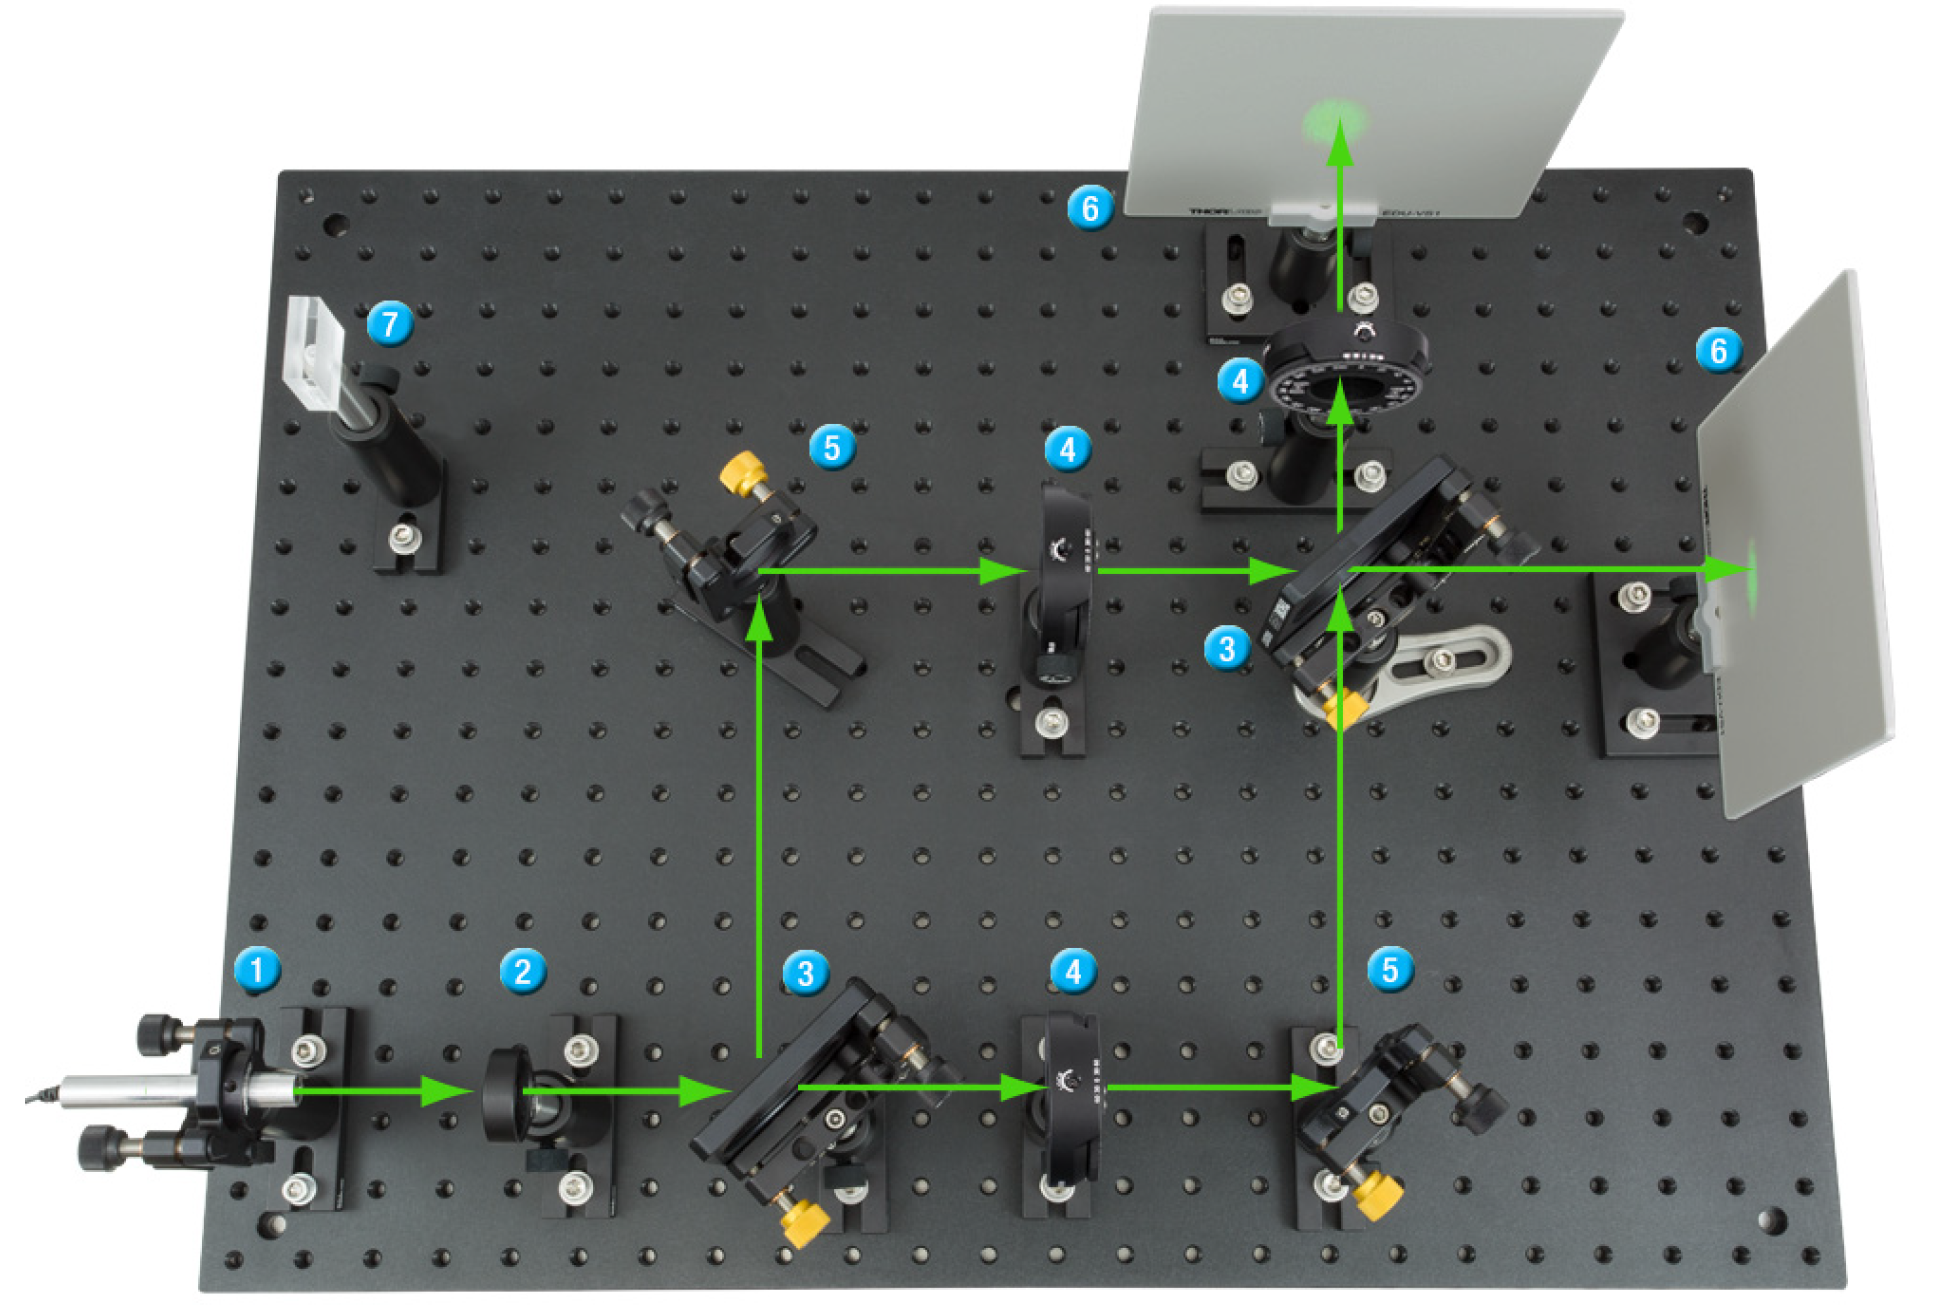
\includegraphics[width=0.8\textwidth]{干涉仪光路图.png}
    \captionof{figure}{干涉仪光路图}
\end{minipage}
\end{document}